% !TEX TS-program = pdflatex
% !TEX encoding = UTF-8 Unicode

% This is a simple template for a LaTeX document using the "article" class.
% See "book", "report", "letter" for other types of document.

\documentclass[11pt]{article} % use larger type; default would be 10pt

\usepackage[utf8]{inputenc} % set input encoding (not needed with XeLaTeX)

%%% Examples of Article customizations
% These packages are optional, depending whether you want the features they provide.
% See the LaTeX Companion or other references for full information.

%%% PAGE DIMENSIONS
\usepackage{geometry} % to change the page dimensions
\geometry{a4paper} % or letterpaper (US) or a5paper or....
% \geometry{margin=2in} % for example, change the margins to 2 inches all round
% \geometry{landscape} % set up the page for landscape
%   read geometry.pdf for detailed page layout information

\usepackage{graphicx} % support the \includegraphics command and options
\usepackage{amsmath}
\usepackage{amsfonts}

% \usepackage[parfill]{parskip} % Activate to begin paragraphs with an empty line rather than an indent

%%% PACKAGES
\usepackage{booktabs} % for much better looking tables
\usepackage{array} % for better arrays (eg matrices) in maths
\usepackage{paralist} % very flexible & customisable lists (eg. enumerate/itemize, etc.)
\usepackage{verbatim} % adds environment for commenting out blocks of text & for better verbatim
\usepackage{subfig} % make it possible to include more than one captioned figure/table in a single float
% These packages are all incorporated in the memoir class to one degree or another...

%%% HEADERS & FOOTERS
\usepackage{fancyhdr} % This should be set AFTER setting up the page geometry
\pagestyle{fancy} % options: empty , plain , fancy
\renewcommand{\headrulewidth}{0pt} % customise the layout...
\lhead{}\chead{}\rhead{}
\lfoot{}\cfoot{\thepage}\rfoot{}

%%% SECTION TITLE APPEARANCE
\usepackage{sectsty}
\allsectionsfont{\sffamily\mdseries\upshape} % (See the fntguide.pdf for font help)
% (This matches ConTeXt defaults)

%%% ToC (table of contents) APPEARANCE
\usepackage[nottoc,notlof,notlot]{tocbibind} % Put the bibliography in the ToC
\usepackage[titles,subfigure]{tocloft} % Alter the style of the Table of Contents
\renewcommand{\cftsecfont}{\rmfamily\mdseries\upshape}
\renewcommand{\cftsecpagefont}{\rmfamily\mdseries\upshape} % No bold!

%%% END Article customizations

%%% The "real" document content comes below...

\title{Project 3 - Mastery Question}
\author{Tom McGrath}
%\date{} % Activate to display a given date or no date (if empty),
         % otherwise the current date is printed 

\begin{document}
\maketitle

\section{Mastery Question}

\subsection{MQ.i.}
I used the Euler-Marayama method to generate a trajectory for the process:
\begin{align}
	dX_{t} &= (\mu - \nu_{t}/2)dt + \sigma_{t}dW^{1}_{t}\\
	d\nu_{t} &= \kappa(\alpha - \nu_{t})dt + \gamma\nu^{\frac{1}{2}}dW^{2}_{t}
\end{align}
where $\mathbb{E}(dW^{1}_{t}dW^{2}_{t})=\rho dt$ and $\sigma^{2}_{t} = \nu_{t}$ with constants $\mu = 0.05$, $\kappa = 5$, $\alpha = 0.04$, $\gamma = 0.5$ and $\rho = -0.5$ on the domain $[0,10]$. This choice of constants satisfies the Feller condition $2\kappa\alpha \geq \gamma^{2}$ (from Ait-Sahalia's paper) so there is in theory no danger of crossing the zero boundary and generating complex-valued results. In practice with a discretisation of $\Delta t = 10^{-3}$ this does occasionally occur. When this happened I re-generated the results.
\newline

I then added noise:
\begin{equation}
	Y_{t_{i}} = X_{t_{i}} + \epsilon_{t_{i}},\quad i = 0,...,N
\end{equation}

with independently distributed noise $\epsilon_{t_{i}} \sim \mathcal{N}(0,0.1)$. A sample trajectory is shown below.
\begin{figure}[h!]
\centering
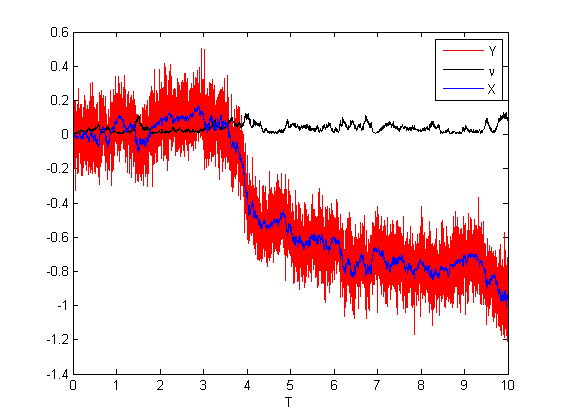
\includegraphics[width = 0.9\textwidth]{MQtraj.png}
\caption{Sample trajectory from the Heston process}
\end{figure}

\subsection{MQ.ii.}
The quadratic variation $\langle Y,Y\rangle$ is given by:
\begin{equation}
	\langle Y,Y \rangle =\lim_{\Delta t_{k} \to 0}|X_{t_{k+1}} - X_{t_{k}}|^{2}
\end{equation}
which gives the drift coefficient as as:
\begin{equation}
	\sigma^{2}_{J} = \frac{1}{J\delta}\sum^{J-1}_{j=0}(X_{j+1}-X_{j})^{2}
\end{equation}
and this converges as $J\to\infty$ to $\sigma^{2}$. Sampling using this method gives the drift coefficient as $0.1$ in the case of using all the data with this estimator. We can obtain the integrated stochastic volatility (ISV) using the equatioin
\begin{equation}
	\lim\sum(X_{t_{i+1}} - X_{t_{i}})^{2} = \int^{T}_{0}\sigma^{2}_{t}dt
\end{equation}
Using different subsampling frequencies alters the ISV as follows:
\begin{figure}[h!]
\centering
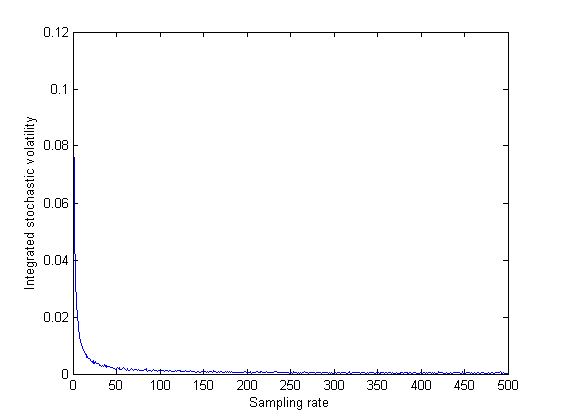
\includegraphics[width = 0.9\textwidth]{MQqv.png}
\caption{Variation of ISV with subsampling frequency}
\end{figure}
I suspect I have made a mistake here - the ISV appears to go to nearly zero as the sampling rate increases and there does not appear to be any indication of optimality. However, the ISV shows the correct behaviour (sampling the noise!) when all of the data is used.
\subsection{MQ.iii.}
We can improve on the subsampling method by using a multi-grid subsampling method, followed by averaging the subsamples. The optimal grid size  is given by:
\begin{equation}
	n_{opt} = \left( \frac{T}{6(\sigma^{2}_{\epsilon})^{2}}\int^{T}_{0}\sigma^{4}_{t}dt\right)^{\frac{1}{3}}
\end{equation}
I chose a grid size of 300. Assigning each point to a grid equidistantly (Ait-Sahalia shows this is optimal in section 4.2 of the paper) the variance of the averaged estimator is calculated to be $2.3477\times 10^{-6}$. This is higher than expected from Ait-Sahalia's table of results (Table 2) which indicates I may have made an error in my code as the parameters chosen are the same.

\subsection{MQ.iv.}
I have not written code for this section as I think I have made a coding error in the previous section. However, all that would be necessary is to subtract the estimate from section ii from the multi-grid variance estimate given by section iii. This gives the first-best estimator and is unbiased as it removes the $2n\sigma^{2}_{\epsilon}$ bias term from the second-best estimator. This could be shown by observing the convergence of mean of the estimator as the number of samples increases.

\section{Code}
\begin{verbatim}
rate = 100;
Tmax = 10;
dt = 0.001;
T = linspace(0,Tmax,Tmax/dt);

mu = 0.05;
kappa = 5;
alpha = 0.04;
gamma = 0.5;
rho = -0.5;

cov = [1,rho;rho,1];

dW = sqrt(dt)*(1/sqrt(2))*cov*randn(2,length(T));
X = zeros(1,length(T));
v = zeros(1,length(T));
Y = zeros(1,length(T));
eta = 0.1*randn(1,length(T));

% generate v
v(1) = 0;
for i = 2:length(T)
   v(i) =  v(i-1) + kappa*(alpha - v(i-1))*dt + sqrt(v(i-1))*gamma*dW(1,i);
end

% generate X
X(1) = 0;
for i = 2:length(T)
    X(i) = X(i-1) + (mu - 0.5*v(i))*dt + sqrt(v(i))*dW(2,i);
end

% generate Y
for i = 1:length(T)
   Y(i) = X(i) + eta(i);
end

qv = 0;
for i = 1:rate:length(T)-rate
    qv = qv+(Y(i+rate)-Y(i))^2;
end

qv = qv/(2*Tmax/dt);
var(X)
var(Y)
qv
sigX = (0.5*dt/Tmax)*sum(diff(X).^2)
sigY = (0.5*dt/Tmax)*sum(diff(Y).^2)
% mean(v)
% 
plot(T,Y, 'Color', 'red')
hold on
plot(T,v, 'Color', 'black')
plot(T,X, 'Color', 'blue')
hold off


function [ qv ] = MQfn( rate )
Tmax = 10;
dt = 0.001;
T = linspace(0,Tmax,Tmax/dt);

mu = 0.05;
kappa = 5;
alpha = 0.04;
gamma = 0.5;
rho = -0.5;

cov = [1,rho;rho,1];

dW = sqrt(dt)*(1/sqrt(2))*cov*randn(2,length(T));
X = zeros(1,length(T));
v = zeros(1,length(T));
Y = zeros(1,length(T));
eta = 0.1*randn(1,length(T));

% generate v
v(1) = 0;
for i = 2:length(T)
   v(i) =  v(i-1) + kappa*(alpha - v(i-1))*dt + sqrt(v(i-1))*gamma*dW(1,i);
end

% generate X
X(1) = 0;
for i = 2:length(T)
    X(i) = X(i-1) + (mu - 0.5*v(i))*dt + sqrt(v(i))*dW(2,i);
end

% generate Y
for i = 1:length(T)
   Y(i) = X(i) + eta(i);
end

Z = zeros(1,floor(length(T)/rate));
for i = 1:length(Z)
   Z(i) = Y(rate*i); 
end

qv = 0.5*dt*sum(diff(Z).^2);

end

function [ qv ] = MQfn2( rate )
Tmax = 10;
dt = 0.001;
T = linspace(0,Tmax,Tmax/dt);

mu = 0.05;
kappa = 5;
alpha = 0.04;
gamma = 0.5;
rho = -0.5;

cov = [1,rho;rho,1];

dW = sqrt(dt)*(1/sqrt(2))*cov*randn(2,length(T));
X = zeros(1,length(T));
v = zeros(1,length(T));
Y = zeros(1,length(T));
eta = 0.1*randn(1,length(T));

% generate v
v(1) = 0;
for i = 2:length(T)
   v(i) =  v(i-1) + kappa*(alpha - v(i-1))*dt + sqrt(v(i-1))*gamma*dW(1,i);
end

% generate X
X(1) = 0;
for i = 2:length(T)
    X(i) = X(i-1) + (mu - 0.5*v(i))*dt + sqrt(v(i))*dW(2,i);
end

% generate Y
for i = 1:length(T)
   Y(i) = X(i) + eta(i);
end

grids = zeros(1,rate);

for i = 1:rate
   for j = i:rate:(length(T)-rate)
      grids(i) = grids(i) + (Y(j+rate)-Y(j))^2;
   end
end

qv = mean(grids);
qv = rate*qv/(2*Tmax/dt);

end

\end{verbatim}


\end{document}
